\documentclass[main.tex]{subfiles}
\begin{document}


\chapter{Fazit}

Aus den erstellten Prototypen und der Evaluation sind Erkenntnisse zusammengekommen, die hier noch zusammengefasst werden. 


\section{Performance}
Aus den Messungen der Performance mittels JMeter haben sich einige Resultate  bezüglich Durchsatz, Latenzzeit und Verfügbarkeit ergeben.


\subsection{Durchsatz}
% Welcher der Services hat am Meisten Durchsatz an den Tag gelegt ? 

Der höchste Durchsatz wurde mit Apache PDFBox erreicht, gefolgt von iText und dann JasperReports. Die Analyse des Durchsatzes nach Bytes hat jedoch ergeben, JasperReports die kleinsten PDFs erstellt die schneller zu übertragen sind. 

\subsection{Latenzzeit}
Auch bei der 'Latency by Request' ist Apache PDFBox am schnellsten. Die Verarbeitung kann bei den ersten zwei Szenarien unterhalb einer Sekunde durchgeführt werden, was bei JasperReports nicht der Fall ist. iText wiederum hat nur leicht längere Latenzzeiten.

\subsection{Verfügbarkeit}

Keiner der Tests ist jemals ausgefallen. Es haben sich auch keine Fehler ereignet, die von JMeter als solche identifiziert wurden. Die meisten Tests haben sich über die Zeitspanne von 10 Stunden erstreckt. Dabei haben die Logdateien ebenfalls keine Ausfälle nachgewiesen.

Dennoch hat JasperReports sehr lange Antwortzeiten, die ebenfalls zu Timeouts führen könnten, was somit die Verfügbarkeit einschränkt.


\section{Ressourcen}
Die Logdateien auf dem PaaS zeichneten den Verbauch von Memory und CPU-Last auf. JasperReport wird als einen starken Ressourcen-Nutzer beurteilt.  
\subsection{Arbeitsspeicher}
Der Verbrauch von RSS-Memory ist sowohl bei iText als auch bei Apache PDFBox meist unterhalb der Memory-Quota. Der SWAP wird einzig von JasperReports stark genutzt und erklärt unter anderem die lange Verarbeitungszeit. Der SWAP wird nicht wieder freigegeben, was zu einer Memory-Blase führen kann.

\subsection{Prozessor Last}
Die CPU Last hat nur bei JasperReports durchgängige Spitzen angezeigt. Apache PDFBox hat hier ressourcenschonend gearbeitet. iText hat eine nicht erklärbare tiefe CPU Last im Szenario 3.


\section{Wer hat nun die beste Performance?}

\begin{figure}[!hb]
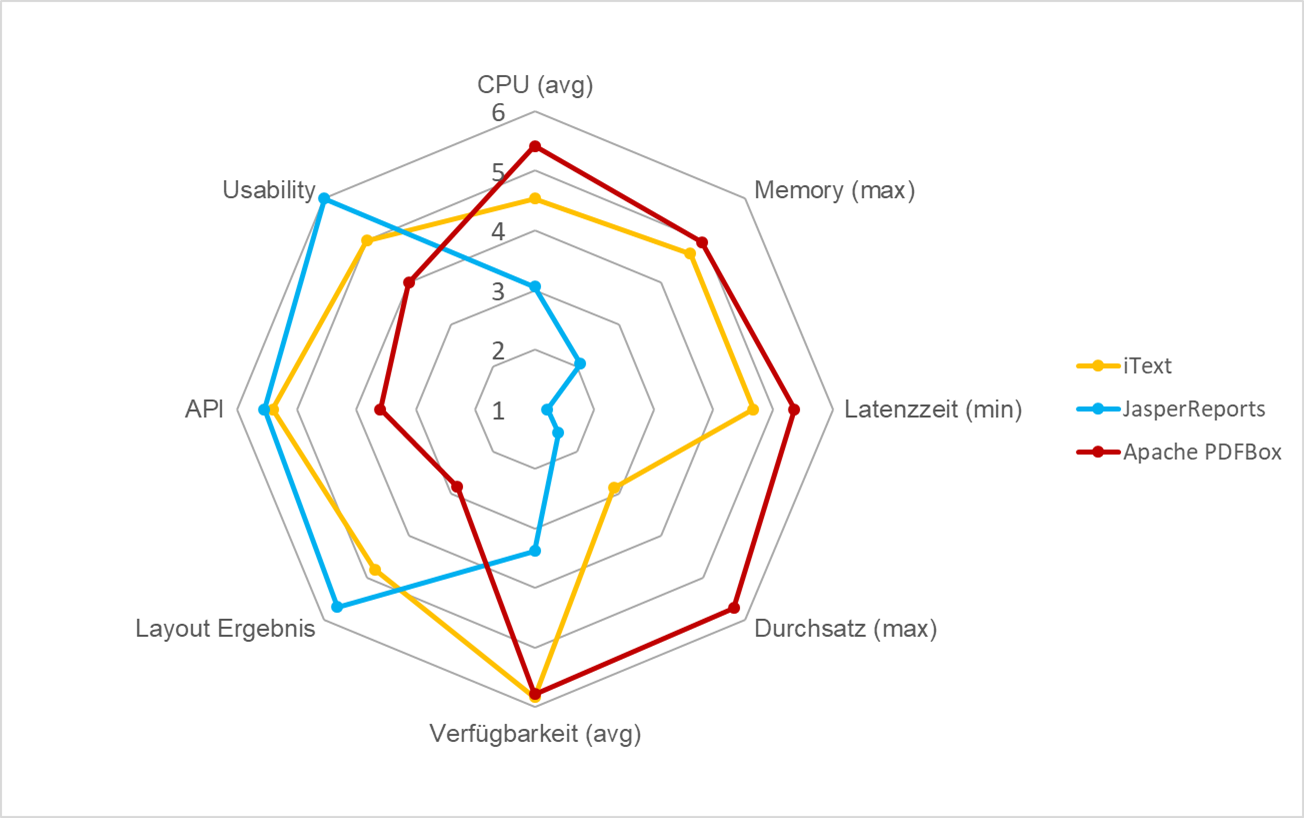
\includegraphics[width=\textwidth]{end/5_erfarhungsbericht/Netzdiagram.png}
 \caption{Netzdiagramm nach Metrik}
 \label{figure:netzdiagrammMetriken}
\end{figure}

Würde man für diese Frage einzig und alleine die Daten des Durchsatzes nehmen, müsste man sagen, es sei im Durchschnitt Apache PDFBox. Dies ist aber nur ein Indiz. Trotz des Szenarios 3 erreicht dieser immer noch durchschnittlich 70 Anfragen pro Sekunde, gefolgt von iText mit 30 Anfragen pro Sekunde und dann JasperReports mit 14.5 Anfragen pro Sekunde.

Die Latenzzeit hat wiederum gezeigt, dass JasperReports der schnellste ist und das nur, weil das Szenario 3 die Antwortzeiten der beiden anderen \acrshort{osre} in die Höhe getrieben hat.

Als Hinweis lässt sich sagen, dass sich im besten Fall mit Apache PDFBox die höchste Performanz und beste Ressourcennutzung sowie Antwortzeiten erreichen lassen. Dennoch haben auch die anderen \acrshort{osre}s gute Seiten, die in verschiedenen Anwendungsfällen besser einzusetzen sind. Im Netzdiagramm lassen sich die Tendenzen der jeweiligen \acrshort{osre} erkennen (siehe Abbildung \ref{figure:netzdiagrammMetriken}).

\subsection{Apache PDFBox}
Diese hat klare Stärken, was die technische Performance angeht. Die Umsetzung ist klar auch historisch geprägt. Es ist ein Tool primär zur Extraktion von Daten und nicht für die Erstellung von Reports gedacht, was es auch so performant macht. Das geeignete Einsatzgebiet im Umfeld von Reporterstellung liegt auf dem Gebiet von statischen Layouts wie Flugtickets oder Konzertkarten. Für dynamische oder kunstvolle Dokumenten-Layouts ist diese Library eher nicht geeignet. 


\subsection{iText}

iText wurde genau dafür kreiert, um Reports zu generieren. Dies ist klar erkennbar an dem versatillen und umfangreichen API. Es beherrscht auch den komplexeren PDF-Aufbau ohne Performance-Verlust. Für einen Online-Einsatz wird es als brauchbar gewertet. Das API ist gut genug, um Reports leicht verständlich zu codieren und bleibt darum wartbar. Der Verbrauch von Ressourcen und die gelieferten Antwortzeiten sind gut. 



\subsection{JasperReports}
Es gibt klare Vorteile bei visuell aufbereiteten Reports. Leider hat aber dieser Vorteil keine nutzbare Performance für eine Online-Verarbeitung gezeigt. Dies bedeutet: JasperReports ist für einen Einsatz in einem Microservice nur sehr bedingt geeignet. Ein geeignetes Einsatzgebiet wären zeitlich klar definierte Reportgenerierungen. Oder auch wenn komplexe Reports womöglich von Nicht-Entwicklern definiert werden sollen, ist iReport dafür ein geeignetes Hilfsmittel. JasperReports kann möglicherweise auf eine bessere Performance getrimmt werden und kann sicherlich in der Anwendung verbessert werden. 

\section{Ausblick}

Aus den Performance-Messungen entstanden einige Fragen im Zusammenhang mit der Implementation, die noch zu adressieren sind, wie z.B.: 
\begin{itemize}  
    \item Sind Engpässe in Applikation oder I/O Ursachen für die schlechte Performance? 
    \item Sind Mängel in der Applikation vorhanden, die einen unnötigen Programmcode ausführen? 
\end{itemize}
Und in dieser Arbeit nicht addressierbare Fragen bezüglich Skalierbarkeit der PaaS.
\begin{itemize}  
    \item Mit welcher Anzahl Server können X Anzahl User performant bedient werden?
    \item Wie verhält sich das Auto-Scaling?
    \item Wie gut funktioniert das Load Balancing ? 
\end{itemize}
Diese Fragen könnten in einer weiteren Arbeit vertieft werden. 

\end{document}